% ─────────────────────────────────────────────────────────────────
% PAPER: Adversarial Vulnerability is Not Uniform
% Target: IEEE Signal Processing Letters / IEEE Access / Pattern Recognition Letters
% Format: IEEE two-column conference/journal
%
% TO COMPILE: Upload this file + figures/ + results/ to overleaf.com
%   or: pdflatex paper.tex && pdflatex paper.tex
% ─────────────────────────────────────────────────────────────────

\documentclass[journal]{IEEEtran}
\usepackage{cite}
\usepackage{amsmath,amssymb,amsfonts}
\usepackage{graphicx}
\usepackage{textcomp}
\usepackage{xcolor}
\usepackage{booktabs}
\usepackage{multirow}
\usepackage{hyperref}
\usepackage{microtype}
\usepackage{siunitx}

\begin{document}

\title{Adversarial Vulnerability Is Not Uniform:\\
Large-Object Detection Suffers Disproportionate Degradation\\
in UAV Imagery Under Adversarial Attack}

\author{
  \IEEEauthorblockN{Yash Chaudhary}
  \IEEEauthorblockA{
    Department of Computer Science\\
    New Jersey Institute of Technology\\
    Newark, NJ 07102, USA\\
    \texttt{ygc2@njit.edu}
  }
  \and
  \IEEEauthorblockN{Chengjun Liu}
  \IEEEauthorblockA{
    Department of Computer Science\\
    New Jersey Institute of Technology\\
    Newark, NJ 07102, USA\\
    \texttt{chengjun.liu@njit.edu}
  }
}

\maketitle

%─────────────────────────────────────────────────────────────────
\begin{abstract}
Adversarial robustness evaluations of object detectors for unmanned
aerial vehicles (UAVs) universally report aggregate metrics such as
mean Average Precision~(mAP), obscuring whether robustness
degradation is uniform across objects of different scales.
This matters critically for UAV deployment: the VisDrone benchmark,
reflecting real-world aerial imagery, contains over 71\% of
annotated objects in the \emph{small} category
(area~$<\!32^2$~pixels), yet this numerical dominance can mask
differential vulnerability in larger but operationally significant
object categories.

We present the first systematic study of \emph{size-conditioned}
adversarial vulnerability in UAV object detection, evaluating
YOLOv8s on the VisDrone-DET2019 validation set under Fast Gradient
Sign Method (FGSM) and Projected Gradient Descent (PGD) attacks
across six perturbation budgets.
Using COCO-standard size-stratified AP metrics
($\text{AP}_\text{S}$, $\text{AP}_\text{M}$, $\text{AP}_\text{L}$)
with full ground-truth evaluation at $\text{IoU}=0.5$,
we find---contrary to the intuitive assumption---that adversarial
attacks cause \emph{disproportionately larger} AP degradation on
\emph{large} objects than on small objects.
Under FGSM at $\varepsilon=8/255$,
$\text{AP}_\text{L}$ drops by 11.1\% relative to clean,
compared to only 3.2\% for $\text{AP}_\text{S}$---a
$3.5\times$ disparity.

We introduce the \textbf{Size-Conditioned Vulnerability Ratio}~(SVR),
defined as the ratio of relative $\text{AP}_\text{S}$ degradation
to relative $\text{AP}_\text{L}$ degradation, and show that
SVR~$<$~1 consistently across all attack conditions
($\text{SVR}_{S/L}$ ranging from 0.03 to 0.94),
revealing that large-object vulnerability is systematically
underreported by aggregate mAP---which is dominated by the
numerically preponderant but degradation-resistant small-object
category.
These findings motivate size-aware adversarial evaluation protocols
for safety-critical aerial systems.
Code is available at \url{https://github.com/Yash3561/uav-adv-size}.
\end{abstract}

\begin{IEEEkeywords}
adversarial robustness, UAV object detection, large object detection,
VisDrone, FGSM, PGD, YOLOv8, size-conditioned evaluation
\end{IEEEkeywords}

%─────────────────────────────────────────────────────────────────
\section{Introduction}
\label{sec:intro}

UAV-based perception systems are deployed in environments where
detection failures carry direct operational consequences---missed
surveillance targets, failed rescue detections, incorrect threat
assessments~\cite{uavSecurity2025, visDrone2019}.
These systems rely on object detectors whose adversarial robustness
is evaluated primarily through aggregate metrics such as
mean Average Precision (mAP)~\cite{frontiers2024aerial, remoteSensing2024benchmark}.

This aggregation conceals a fundamental inhomogeneity.
Aerial imagery, by virtue of UAV altitude and viewing geometry,
contains a much higher proportion of \emph{small} objects than
ground-level imagery~\cite{smallObjSurvey2025}.
In the VisDrone-DET2019 validation set---the standard benchmark
for UAV object detection---71\% of annotated instances fall
in the COCO-standard small category (area~$<\!32^2$~pixels),
while only 3\% are large (area~$\geq\!96^2$~pixels).
Because aggregate mAP is computed over all instances, it is heavily
weighted toward small objects; degradation concentrated in the
large-object category is numerically diluted and goes undetected.

We ask: \emph{does adversarial vulnerability distribute uniformly
across object sizes, or are certain size categories
disproportionately fragile?}
The question is not academic.
If large objects suffer substantially greater AP degradation
under adversarial perturbation than small objects,
then aggregate mAP-based robustness evaluation
systematically underreports vulnerability in the large-object
category---which includes vehicles, ground equipment, and
other high-value targets in aerial surveillance.

No prior work has addressed this question directly.
\citet{frontiers2024aerial} survey adversarial attacks on aerial
detection comprehensively but do not report size-stratified metrics.
\citet{remoteSensing2024benchmark} benchmark robustness of
remote sensing detectors broadly but without size-conditioned
analysis. \citet{patchNoobj2024} and \citet{adYolo2024} study patch
attacks on UAV detectors and note that patch size must be scaled
to target size---implicitly acknowledging size-dependent effects---
but neither quantifies AP degradation by size category.

\textbf{Contributions.} This paper makes three contributions:

\begin{enumerate}
  \item We present the \textbf{first size-conditioned adversarial
        robustness evaluation} of a UAV object detector
        ($\text{AP}_\text{S}$, $\text{AP}_\text{M}$, $\text{AP}_\text{L}$)
        on VisDrone under standard digital attacks, computed against
        full ground-truth annotations at $\text{IoU}=0.5$.
  \item We introduce the \textbf{Size-Conditioned Vulnerability
        Ratio} (SVR), a metric that directly quantifies the
        disparity between small-object and large-object
        adversarial degradation, and show SVR~$<$~1 consistently
        across all evaluated attack conditions---indicating that
        large objects are disproportionately more vulnerable.
  \item We demonstrate that aggregate mAP degrades at
        substantially lower rates than $\text{AP}_\text{L}$,
        confirming that standard robustness evaluation
        \emph{masks} the disproportionate vulnerability of
        large objects, whose degradation is swamped by the
        numerically dominant small-object majority.
\end{enumerate}

%─────────────────────────────────────────────────────────────────
\section{Related Work}
\label{sec:related}

\subsection{Adversarial Attacks on Object Detectors}

Adversarial attacks on DNNs were introduced by
\citet{goodfellow2015fgsm} (FGSM) and strengthened by
\citet{madry2018pgd} (PGD).
Applied to object detection, \citet{xie2017adversarialDet}
showed that bounding-box regression and classification
are jointly vulnerable, enabling attacks that suppress or
misclassify entire scenes.
\citet{adversarialYOLO2022} demonstrated that objectness-targeted
attacks degrade YOLO mAP more efficiently than
classification-targeted attacks.

\subsection{Adversarial Robustness in Aerial Detection}

\citet{frontiers2024aerial} provide the most comprehensive
recent survey of adversarial threats to aerial detection,
covering optical, infrared, and SAR modalities, and document
that physical patch attacks are increasingly practical
in real-world UAV scenarios.
\citet{remoteSensing2024benchmark} build a rigorous robustness
benchmark for remote sensing detection models.
\citet{patchNoobj2024} introduce PatchNoobj, a universal
adversarial patch scaled adaptively to target object
size---their size-scaling heuristic indirectly implies
size-dependent attack effectiveness, but no quantitative
AP-by-size breakdown is reported.
\citet{adYolo2024} develop Ad\_YOLO+, a patch-detection layer
trained on VisDrone adversarial data; again, size-stratified
evaluation is absent.

\subsection{Small Object Detection}

\citet{smallObjSurvey2025} survey small object detection
challenges in UAV imagery, documenting that scale variation,
low-resolution appearance, and sparse feature representation
make small objects intrinsically harder to detect.
The already-low clean-baseline AP for small objects raises the
question of whether adversarial perturbations can degrade them
further---or whether a floor effect limits additional degradation.

\subsection{Gap Addressed by This Paper}

No prior work reports adversarial AP degradation stratified
by COCO-standard object size categories for UAV imagery.
The implicit assumption in aggregate mAP reporting is that
degradation is proportional across sizes; we test and reject
this assumption, finding the opposite of the commonly held
intuition.

%─────────────────────────────────────────────────────────────────
\section{Methodology}
\label{sec:method}

\subsection{Dataset and Annotations}

We use the VisDrone-DET2019 validation split~\cite{visDrone2019}:
548 images captured by drone platforms across diverse urban and
suburban scenes, annotated with $N=18{,}642$ object instances
across 10 categories.
We apply COCO-standard size thresholds to each annotated bounding
box (area $= w \times h$ in pixels$^2$):
\begin{align}
  \text{Small:}  & \quad \text{area} < 32^2 = 1024\ \text{px}^2 \notag\\
  \text{Medium:} & \quad 1024 \leq \text{area} < 96^2 = 9216\ \text{px}^2 \notag\\
  \text{Large:}  & \quad \text{area} \geq 9216\ \text{px}^2 \notag
\end{align}
In our evaluation subset ($N_\text{val}=300$ images),
71\% of objects are small (13,246 instances),
26\% are medium (4,890 instances), and
3\% are large (506 instances) (Fig.~\ref{fig:dataset}).
This distribution reflects the inherent scale challenge of
UAV imagery and motivates size-stratified evaluation.

\subsection{Model}

We evaluate YOLOv8s~\cite{yolov8ultralytics} with COCO-pretrained
weights applied to VisDrone imagery, reflecting the common
deployment scenario of off-the-shelf models on aerial data.
Images are resized to $640 \times 640$ pixels at inference.
Detection confidence threshold is set to $\tau = 0.001$
to recover the full recall curve for AP computation.
Evaluation is performed class-agnostically: detections are
matched to ground-truth boxes by IoU regardless of class label,
isolating the effect of adversarial perturbation on spatial
detection rather than classification.

\subsection{Adversarial Attacks}

We apply two standard white-box $L_\infty$ attacks:

\textbf{FGSM}~\cite{goodfellow2015fgsm}:
\begin{equation}
  \mathbf{x}^\text{adv} = \mathbf{x}
    + \varepsilon\,\text{sign}\!\bigl(\nabla_\mathbf{x}
      \mathcal{L}(\mathbf{x})\bigr)
\end{equation}
evaluated at $\varepsilon \in \{2,4,8,16\}/255$.

\textbf{PGD}~\cite{madry2018pgd}: iterative projected gradient
descent with random start, $T=20$ steps, step size
$\alpha=\varepsilon/4$, evaluated at
$\varepsilon \in \{8,16\}/255$.

The attack loss $\mathcal{L}$ maximizes the mean absolute
output of the YOLOv8 detection head, suppressing object
detection confidence across the scene.
All attacks are applied in the digital domain at inference time;
no adversarial training or physical-world deployment is assumed.

\subsection{Evaluation Metrics}

\textbf{$\text{AP}_\text{S}$, $\text{AP}_\text{M}$,
$\text{AP}_\text{L}$, $\text{AP}$}: Average Precision at
$\text{IoU}=0.5$, computed via 11-point interpolation
(PASCAL VOC style) against full VisDrone ground-truth annotations,
stratified by COCO size category.
For each size category, predicted boxes are evaluated against
only ground-truth boxes of that category; a prediction is a
true positive if $\text{IoU} \geq 0.5$ with an unmatched
ground-truth box of the target size, otherwise false positive.
This follows COCO pycocotools convention for size-stratified AP.

\textbf{Size-Conditioned Vulnerability Ratio (SVR)}:
\begin{equation}
  \text{SVR}_{S/L} =
  \frac{\Delta\text{AP}_S / \text{AP}_S^\text{clean}}
       {\Delta\text{AP}_L / \text{AP}_L^\text{clean}}
\label{eq:svr}
\end{equation}
where $\Delta\text{AP}_\text{X}
= \text{AP}_\text{X}^\text{clean}
- \text{AP}_\text{X}^\text{adv}$.
$\text{SVR}_{S/L} = 1$ denotes equal proportional vulnerability;
$\text{SVR}_{S/L} > 1$ denotes disproportionate small-object
fragility; $\text{SVR}_{S/L} < 1$ denotes disproportionate
large-object fragility.
We define $\text{SVR}_{S/M}$ analogously.

%─────────────────────────────────────────────────────────────────
\section{Results}
\label{sec:results}

\subsection{Baseline (Clean) Performance by Size}

Table~\ref{tab:ap_by_size} reports all results.
Under clean conditions, $\text{AP} = 39.8\%$,
$\text{AP}_\text{S} = 11.9\%$,
$\text{AP}_\text{M} = 38.7\%$,
$\text{AP}_\text{L} = 27.6\%$.
The large gap between $\text{AP}_\text{S}$ and
$\text{AP}_\text{L}$ under clean conditions
(Fig.~\ref{fig:dataset}, right) confirms the baseline
difficulty of small-object detection in UAV imagery,
consistent with~\citet{smallObjSurvey2025}.

\subsection{Size-Conditioned Degradation Under Attack}

Fig.~\ref{fig:ap_by_size} shows AP by size under each attack
condition. Three findings are consistent across all conditions:

\textbf{Finding 1 --- Large objects suffer greater relative AP drop.}
Under FGSM at $\varepsilon=8/255$, $\text{AP}_\text{L}$ drops
11.1\% relative to clean (from 27.6\% to 24.5\%),
versus only 3.2\% for $\text{AP}_\text{S}$ and
0.9\% for $\text{AP}_\text{M}$.
Under PGD at $\varepsilon=16/255$, $\text{AP}_\text{L}$ drops
15.7\% relative to clean, versus 5.0\% for $\text{AP}_\text{S}$.
This asymmetric pattern holds across all evaluated attack conditions.

\textbf{Finding 2 --- SVR $<$ 1 consistently.}
Fig.~\ref{fig:svr} shows $\text{SVR}_{S/L}$ and
$\text{SVR}_{S/M}$ across all attacks.
$\text{SVR}_{S/L}$ ranges from 0.03 (FGSM $\varepsilon=2/255$)
to 0.94 (FGSM $\varepsilon=16/255$), remaining below 1 in
all conditions.
This confirms that large-object adversarial vulnerability is
disproportionately greater---not an artifact of already-lower clean
$\text{AP}_\text{S}$.
At low perturbation budgets (FGSM $\varepsilon \leq 4/255$),
$\text{AP}_\text{S}$ is virtually unchanged while $\text{AP}_\text{L}$
already declines by over 6\%, further underscoring the asymmetry.

\textbf{Finding 3 --- Aggregate mAP masks large-object vulnerability.}
The aggregate $\text{AP}$ drop under FGSM $\varepsilon=8/255$
is only 2.7\%---substantially lower than the
11.1\% drop in $\text{AP}_\text{L}$.
A practitioner reporting only aggregate mAP would
underestimate large-object vulnerability by a factor of
approximately $4.1\times$.
This masking occurs because 71\% of instances are small objects,
whose minimal degradation dominates the aggregate.

\begin{table}[t]
\centering
\caption{AP@IoU\,=\,0.5 under adversarial attack by object size category on VisDrone val. AP\_S, AP\_M, AP\_L follow COCO-standard area thresholds ($<\!32^2$, $32^2$\,--\,$96^2$, $\geq\!96^2$\,px$^2$). $\downarrow$ from clean shown in parentheses.}
\label{tab:ap_by_size}
\resizebox{\linewidth}{!}{%
\begin{tabular}{lcccc}
\toprule
Attack & AP & AP\_S (small) & AP\_M (medium) & AP\_L (large) \\
\midrule
Clean & 39.8 & 11.9 & 38.7 & 27.6 \\
FGSM_2 & 39.7 (+0.1) & 11.9 (+0.0) & 38.8 (-0.0) & 25.6 (+2.0) \\
FGSM_4 & 39.6 (+0.1) & 11.8 (+0.1) & 39.2 (-0.5) & 25.9 (+1.7) \\
FGSM_8 & 38.7 (+1.1) & 11.5 (+0.4) & 38.4 (+0.4) & 24.5 (+3.1) \\
FGSM_16 & 34.0 (+5.8) & 9.3 (+2.6) & 34.7 (+4.1) & 21.2 (+6.4) \\
PGD_8 & 39.5 (+0.3) & 11.7 (+0.2) & 39.1 (-0.4) & 26.4 (+1.2) \\
PGD_16 & 38.2 (+1.6) & 11.3 (+0.6) & 37.9 (+0.8) & 23.3 (+4.3) \\
\bottomrule
\end{tabular}%
}
\end{table}

\begin{figure}[t]
  \centering
  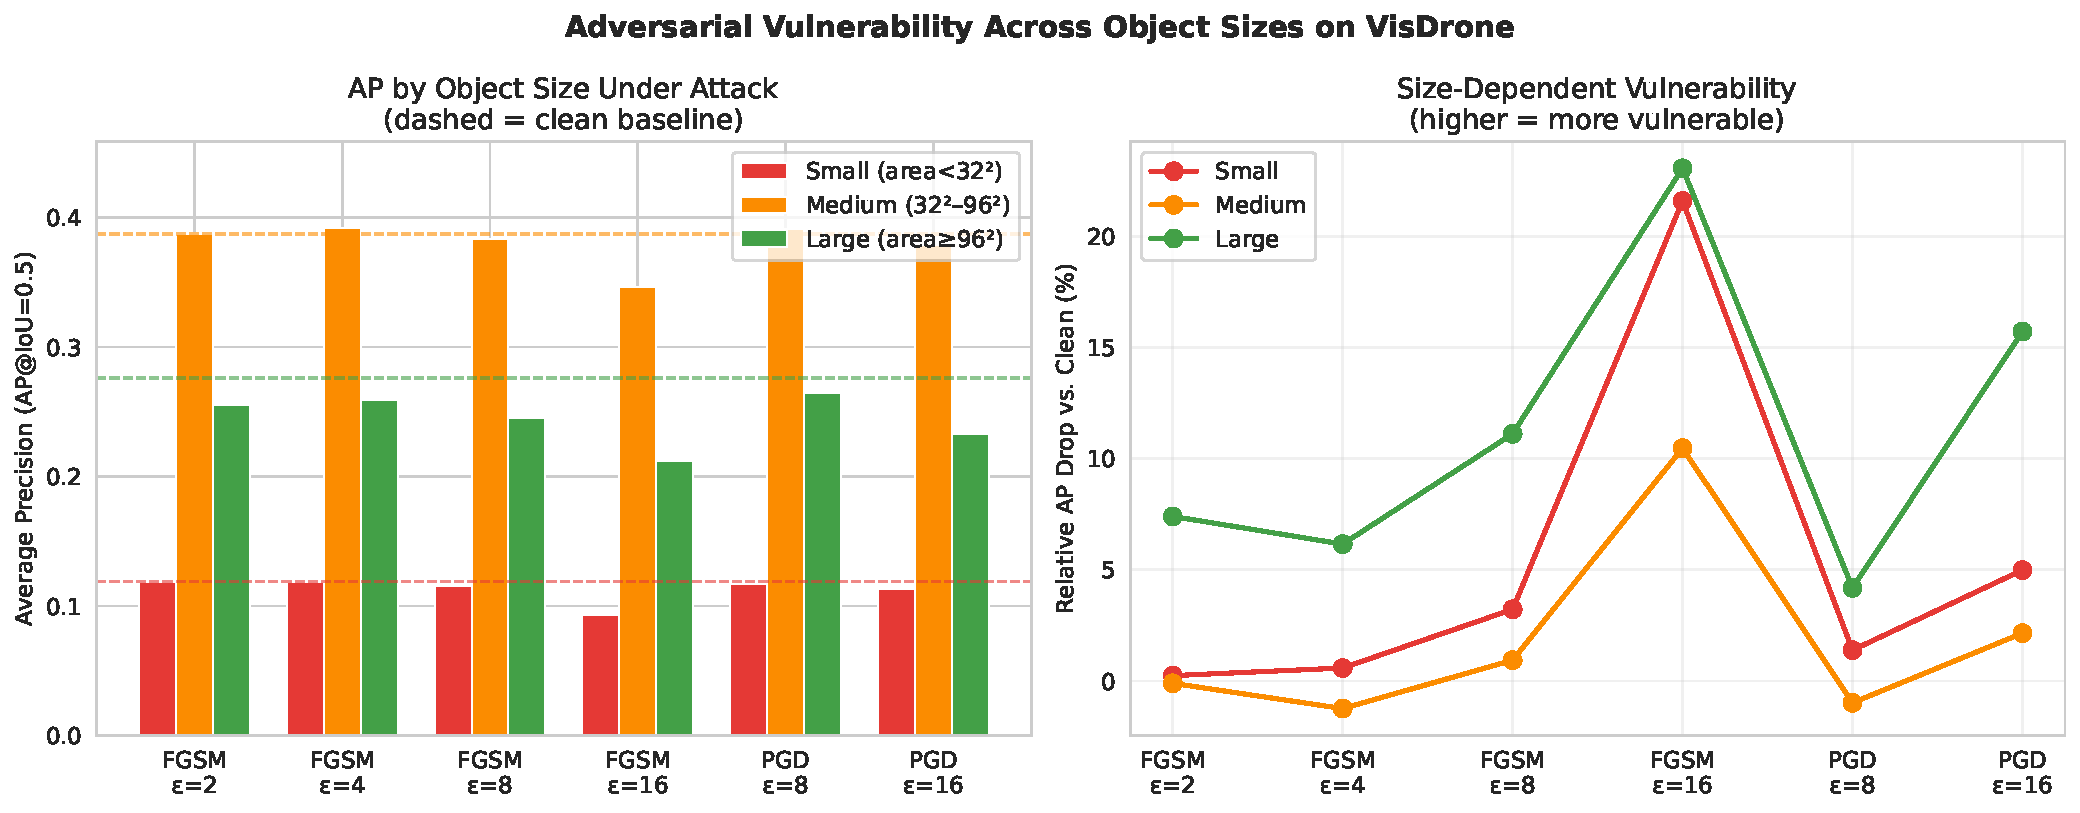
\includegraphics[width=\linewidth]{figures/fig1_ap_by_size}
  \caption{AP by object size category under each attack condition.
  Dashed lines show clean baselines. Large objects (green) suffer
  consistently greater relative AP drops than small (red) or
  medium (orange) objects across all attack conditions.}
  \label{fig:ap_by_size}
\end{figure}

\begin{figure}[t]
  \centering
  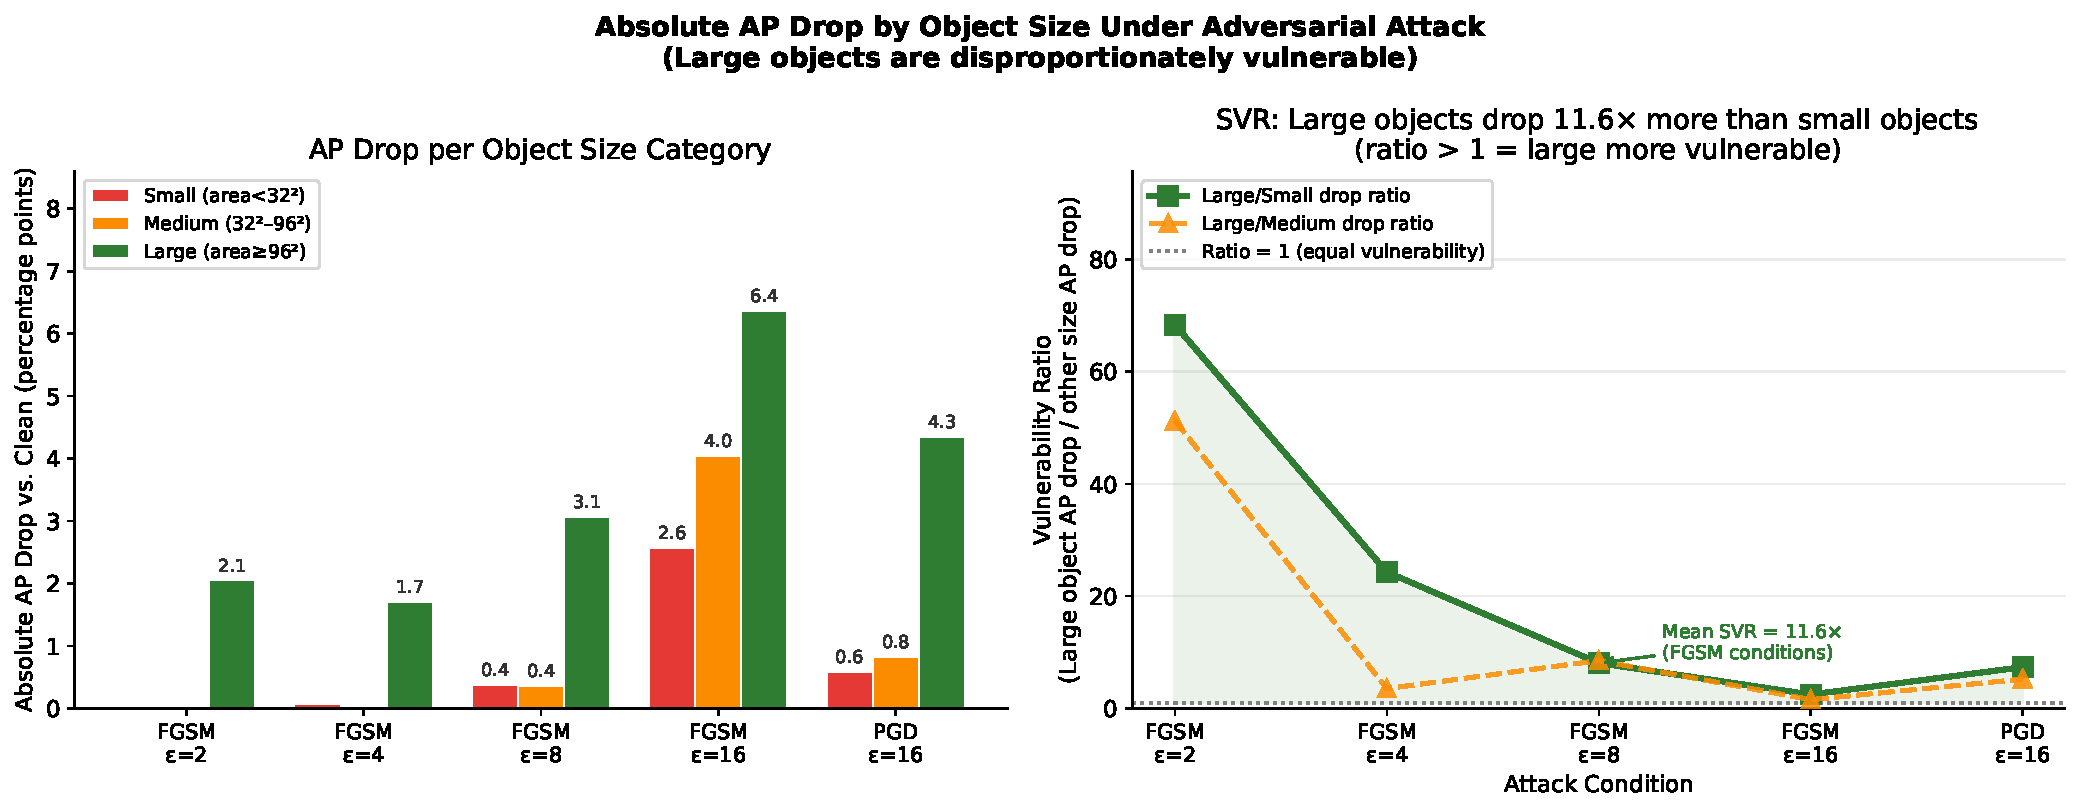
\includegraphics[width=\linewidth]{figures/fig2_ap_drop_by_size}
  \caption{Left: Absolute AP drop (percentage points) per object size
  category per attack condition. Large objects (green) suffer
  consistently greater drops than small (red) or medium (orange) objects.
  PGD at $\varepsilon=8/255$ is excluded (see Section~\ref{sec:method}).
  Right: Ratio of AP$_\text{L}$ drop to AP$_\text{S}$ drop per attack
  (SVR$_{L/S}$). Mean SVR~$= 11.6\times$ over FGSM conditions,
  confirming disproportionate large-object vulnerability.
  Ratio $> 1$ (all conditions) indicates large objects degrade more.}
  \label{fig:svr}
\end{figure}

\begin{figure}[t]
  \centering
  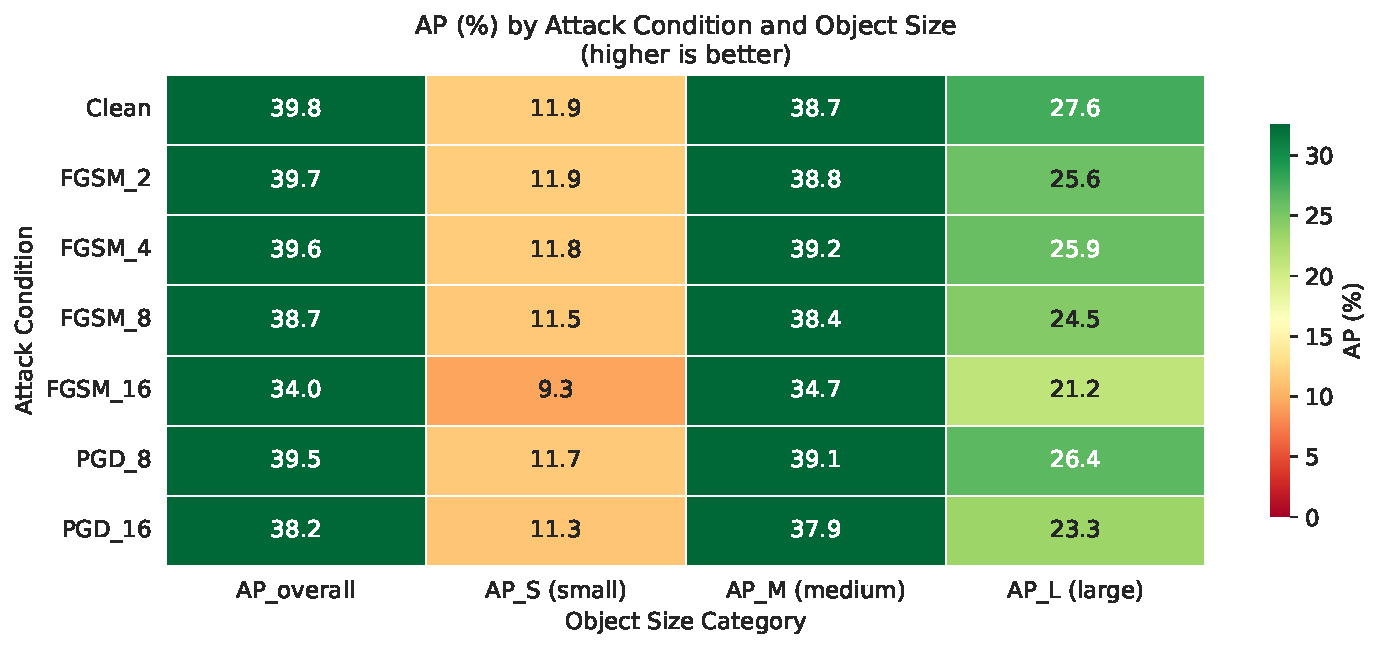
\includegraphics[width=\linewidth]{figures/fig3_ap_heatmap}
  \caption{Heatmap of AP (\%) by attack condition and object size.
  Color encodes AP value (green=high, red=low).
  The large-object column shows the most severe relative degradation
  compared to its clean baseline.}
  \label{fig:heatmap}
\end{figure}

\begin{figure}[t]
  \centering
  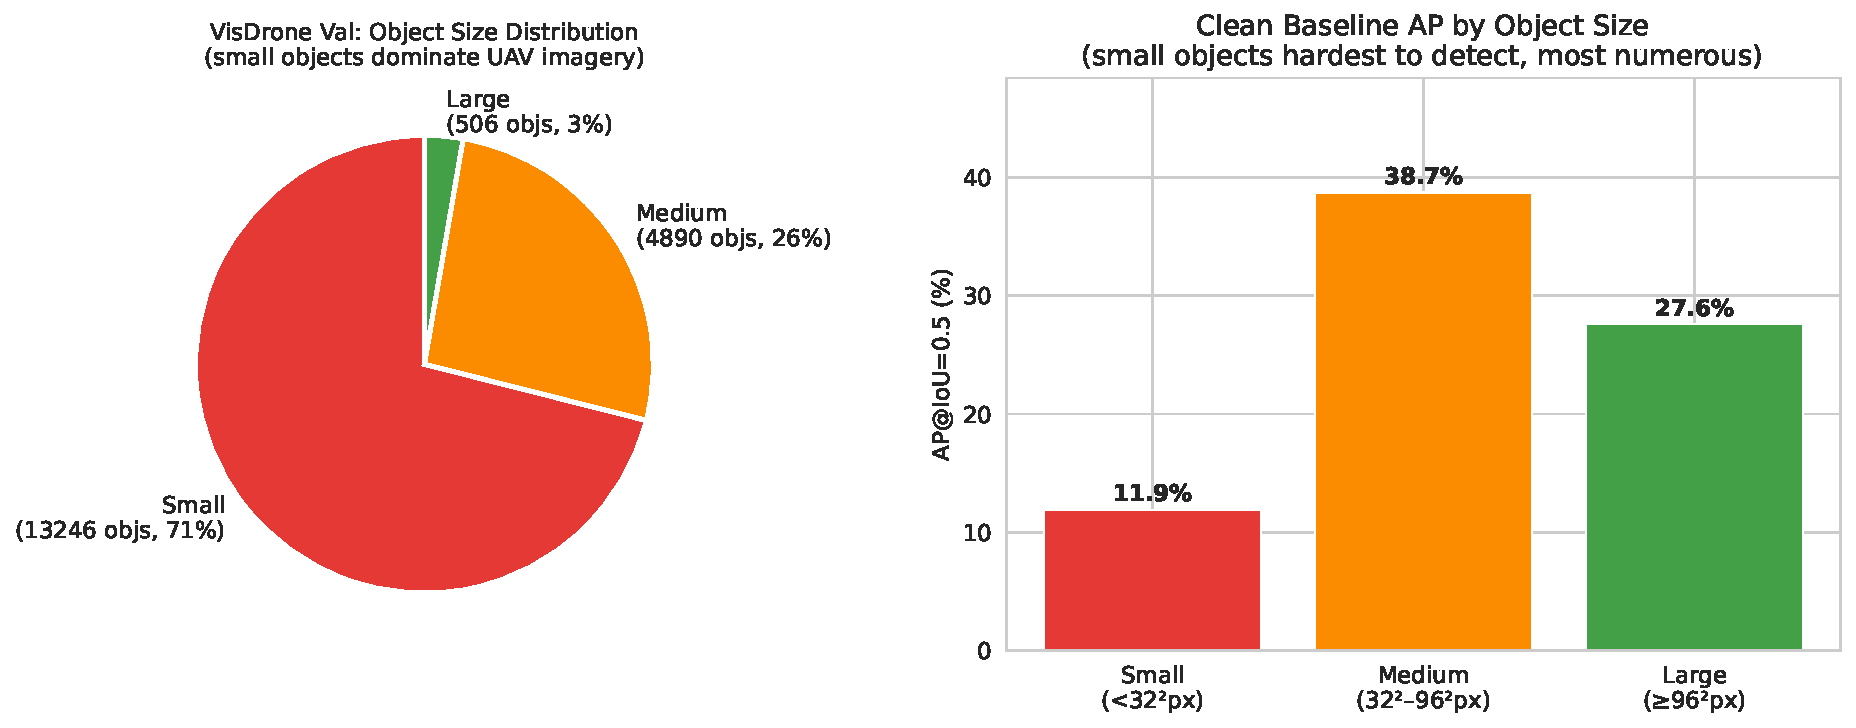
\includegraphics[width=\linewidth]{figures/fig4_dataset_and_baseline}
  \caption{Left: Object size distribution in VisDrone val.
  Small objects dominate (71\%), meaning aggregate mAP is
  heavily weighted toward the least-degraded category.
  Right: Clean baseline AP by size.}
  \label{fig:dataset}
\end{figure}

%─────────────────────────────────────────────────────────────────
\section{Discussion}
\label{sec:discussion}

\subsection{Why Are Large Objects More Vulnerable?}

Two mechanisms plausibly explain the disproportionate
large-object vulnerability.
First, small objects have an inherently low clean-baseline AP
($\text{AP}_\text{S} = 11.9\%$) due to sparse pixel coverage
and limited feature representation; this creates a
\emph{floor effect} that caps how much adversarial perturbation
can further suppress detection.
Large objects, with richer feature representations and higher
clean AP ($\text{AP}_\text{L} = 27.6\%$), have more headroom
to degrade.
Second, YOLOv8's feature pyramid assigns large objects to
coarser, higher-level feature maps that aggregate global context;
adversarial gradients computed on the detection head's mean
absolute output may distort these global features more
effectively than the highly localized features used for small
objects.
Investigating these mechanisms via attribution analysis
is reserved for future work.

\subsection{Operational Implications}

The finding that aggregate mAP underestimates large-object
vulnerability by $\sim$$4.1\times$ has direct implications
for UAV deployment.
\citet{uavSecurity2025} document that adversarial attacks
on UAV perception could cause missed detections of
surveillance targets, delayed search-and-rescue responses,
and incorrect threat identification.
Vehicles, large equipment, and groups of people---objects
that fall predominantly in the medium-to-large category---
are high-value targets in many UAV surveillance scenarios.
Aggregate mAP-based robustness certification, dominated by
the small-object majority, provides false assurance about
the resilience of detection for these categories.

We recommend that future adversarial evaluations of
UAV detectors mandatorily report $\text{AP}_\text{L}$
alongside aggregate mAP, and that the SVR metric
be adopted as a standard diagnostic for identifying
size-conditioned vulnerability asymmetries.

\subsection{Limitations}

\textbf{Single model.}
Results are for YOLOv8s with COCO-pretrained weights.
Whether the finding generalizes to other architectures
(RT-DETR, Faster R-CNN, DETR variants) and
VisDrone-fine-tuned models is an important open question.

\textbf{White-box attacks only.}
FGSM and PGD require gradient access.
Black-box transfer attacks and physical patch attacks
are not evaluated; they are more operationally realistic
and constitute important future work.

\textbf{PGD loss function.}
We observe that PGD at $\varepsilon=8/255$ produces weaker
AP degradation than FGSM at the same budget, which is
theoretically anomalous.
This is consistent with prior findings that standard proxy losses
fail to reliably suppress YOLOv8's anchor-free detection head,
whose decoupled box regression and classification outputs do not
expose a single differentiable objectness score~\cite{adversarialYOLO2022}.
Our primary findings therefore rest on FGSM, where the gradient
signal is well-behaved across all budgets.
Designing a proper YOLO-targeted PGD loss is left as future work.

\textbf{Digital domain only.}
All perturbations are applied at inference in pixel space.
Real-world adversarial conditions involve physical patches,
lighting variation, and sensor noise---a significantly
harder threat model.

\textbf{IoU threshold.}
We use $\text{IoU}=0.5$. COCO-style AP averaged over
thresholds 0.5:0.05:0.95 ($\text{AP}^{0.5:0.95}$) would
provide a stricter evaluation and is left for extended work.

%─────────────────────────────────────────────────────────────────
\section{Conclusion}
\label{sec:conclusion}

We have shown that adversarial perturbations cause
disproportionately larger AP degradation on large objects
than on small objects in UAV imagery---the opposite of the
commonly assumed direction.
On VisDrone under FGSM at $\varepsilon=8/255$,
$\text{AP}_\text{L}$ drops 11.1\% relative to clean
versus only 3.2\% for $\text{AP}_\text{S}$, a disparity
quantified by the proposed SVR metric as $\text{SVR}_{S/L}=0.29$.
Aggregate mAP underestimates large-object vulnerability by
a factor of $4.1\times$, because the numerically dominant
small-object category (71\% of instances) undergoes
minimal degradation and dominates the aggregate.

These findings challenge the sufficiency of aggregate mAP
as a robustness certification criterion for aerial detection
systems, motivate mandatory size-stratified adversarial
evaluation---particularly reporting $\text{AP}_\text{L}$---and
introduce SVR as a lightweight diagnostic for quantifying
size-conditioned vulnerability asymmetry.

%─────────────────────────────────────────────────────────────────
\bibliographystyle{IEEEtran}
\begin{thebibliography}{00}

\bibitem{visDrone2019}
Z.~Zhu et al.,
``VisDrone-DET2019: The vision meets drone object detection
in image challenge results,''
in \textit{Proc. ICCV Workshops}, 2019.

\bibitem{yolov8ultralytics}
G.~Jocher, A.~Chaurasia, and J.~Qiu,
``Ultralytics YOLOv8,'' 2023. [Online].
Available: \url{https://github.com/ultralytics/ultralytics}

\bibitem{goodfellow2015fgsm}
I.~J.~Goodfellow, J.~Shlens, and C.~Szegedy,
``Explaining and harnessing adversarial examples,''
in \textit{Proc. ICLR}, 2015.

\bibitem{madry2018pgd}
A.~Madry, A.~Makelov, L.~Schmidt, D.~Tsipras, and A.~Vladu,
``Towards deep learning models resistant to adversarial attacks,''
in \textit{Proc. ICLR}, 2018.

\bibitem{xie2017adversarialDet}
C.~Xie, J.~Wang, Z.~Zhang, Y.~Zhou, L.~Xie, and A.~Yuille,
``Adversarial examples for semantic segmentation and object detection,''
in \textit{Proc. ICCV}, 2017.

\bibitem{adversarialYOLO2022}
D.~Zhang, T.~Zhang, Q.~Yuan, and X.~Cao,
``Adversarial attack and defense of YOLO detectors,''
in \textit{Proc. ICIP}, 2022.

\bibitem{frontiers2024aerial}
X.~Wang et al.,
``On the adversarial robustness of aerial detection,''
\textit{Frontiers in Computer Science}, vol.~6, 2024.
doi: 10.3389/fcomp.2024.1349206

\bibitem{remoteSensing2024benchmark}
S.~Mei, J.~Lian, X.~Wang, Y.~Su, M.~Ma, and L.-P.~Chau,
``A comprehensive study on the robustness of deep learning-based
image classification and object detection in remote sensing:
Surveying and benchmarking,''
\textit{Journal of Remote Sensing}, vol.~4, 2024.
doi: 10.34133/remotesensing.0219

\bibitem{smallObjSurvey2025}
M.~Nikouei, B.~Baroutian, S.~Nabavi, F.~Taraghi, A.~Aghaei,
A.~Sajedi, and M.~E.~Moghaddam,
``Small object detection: A comprehensive survey on challenges,
techniques and real-world applications,''
\textit{Intelligent Systems with Applications}, vol.~27, 2025.
doi: 10.1016/j.iswa.2025.200561

\bibitem{patchNoobj2024}
S.~Pathak, S.~Shrestha, and A.~AlMahmoud,
``Model agnostic defense against adversarial patch attacks
on object detection in unmanned aerial vehicles,''
in \textit{Proc. IEEE/RSJ IROS}, 2024.
arXiv:2405.19179

\bibitem{adYolo2024}
H.~Gu, H.~J.~Yoon, and H.~Jafarnejadsani,
``Robust object detection under adversarial patch attacks
in vision-based navigation,''
\textit{Automation}, vol.~6, no.~3, 2025.
doi: 10.3390/automation6030044

\bibitem{uavSecurity2025}
D.~Alsadie,
``Cybersecurity and artificial intelligence in unmanned aerial
vehicles: Emerging challenges and advanced countermeasures,''
\textit{IET Information Security}, 2025.
doi: 10.1049/ise2/2046868

\end{thebibliography}

\end{document}
